\documentclass[ba]{imsart}
%
\pubyear{0000}
\volume{00}
\issue{0}
\doi{0000}
%\arxiv{}
\firstpage{1}
\lastpage{1}

\usepackage{subfigure}
\usepackage{amsthm}
\usepackage{amsmath}
\usepackage{amsfonts}
\usepackage{natbib}
\usepackage[colorlinks,citecolor=blue,urlcolor=blue,filecolor=blue,backref=page]{hyperref}
\usepackage{graphicx}

\startlocaldefs
% ** Local definitions **
\endlocaldefs

\begin{document}

%% *** Frontmatter *** 

\begin{frontmatter}
\title{Bayesian Inference for Cox Proportional Hazard Models with Partial Likelihoods, Semi-Parametric Covariate Effects and Correlated Observations}

%\title{\thanksref{T1}}
%\thankstext{T1}{<thanks text>}
\runtitle{}

\begin{aug}
%\author{\fnms{} \snm{}}
%\author{\fnms{<firstname>} \snm{<surname>}\thanksref{}\ead[label=e1]{}}
%\and
%\author{\fnms{} \snm{}}
\author{\fnms{Ziang} \snm{Zhang}},
\author{\fnms{Alex} \snm{Stringer}}
\author{\fnms{Patrick} \snm{Brown}}
\and
\author{\fnms{James} \snm{Stafford}}%


\runauthor{Zhang et al.}

\address[addr1]{}


%\thankstext{<id>}{<text>}

\end{aug}

\begin{abstract}
In this paper, we introduce a novel approximate Bayesian inference methodology for the Cox Proportional Hazard model with partial likelihood that allows the inclusion of linear covariate effects, semi-parametric covariate effects and correlated survival times. The existing method for approximate Bayesian inference for Cox Proportional Hazard model (Integrated Nested Laplace Approximations, INLA), uses full likelihood instead of partial likelihood, and hence requires parametric or a smooth semi-parametric baseline hazard function. Combing the use of a generalization of the Laplace approximation method used in the existing methods with the use of quasi-Newton type of optimization, we propose a way to do approximate Bayesian inference for Cox Proportional Hazard model using partial likelihood, that does not require any assumption on the form of the base hazard function. From a few simulation studies with different types of underlying baseline hazard function, We show that our proposed method provides accurate inference even when the sample size is relatively small. We then utilize our proposed method to re-analyse the dataset of Leukaemia survival times and the dataset of Kidney infection times. An R package implementing our method will be released publicly.
\end{abstract}

%% ** Keywords **
\begin{keyword}
\kwd{Cox Proportional Hazard Model}
\kwd{Partial Likelihood}
\kwd{Approximate Bayesian inference}
\kwd{Semi-parametric Smoothing}
\end{keyword}

\end{frontmatter}

%% ** Mainmatter **

%\section{}\label{}

% \begin{figure} 
% \includegraphics{<eps-file>}% place <eps-file> in ./img  subfolder
% \caption{}
% \label{}
% \end{figure}


% \begin{table} 
% *****************
% \begin{tabular}{lll}
% \end{tabular}
% *****************
% \caption{}
% \label{}
% \end{figure}

%%%%%%%%%%%%%%%%%%%%%%%%%%%%%%%%%%%%%%%%%%%%%%
%% Supplementary Material, if any, should   %%
%% be provided in {supplement} environment  %%
%% with title and short description.        %%
%%%%%%%%%%%%%%%%%%%%%%%%%%%%%%%%%%%%%%%%%%%%%%
%\begin{supplement}
%\stitle{???}
%\sdescription{???.}
%\end{supplement}

%% ** The bibliograhy **
%\bibliographystyle{ba}
%\bibliography{<bib-data-file>}% place <bib-data-file> in ./bib folder 

% ** Acknowledgements **
% \begin{acknowledgement}
% \end{acknowledgement}

\section{Introduction}\label{sec1}
For problems involving time-to-event data, the combination of Cox proportional hazard (Cox PH) models and inference via partial likelihood has been the dominant methodology following its development by Cox \citep{coxph}. The Cox PH model assumes that any two subjects' event hazards are proportional as a function of time, with the ratio depending on unknown linear or smooth covariate effects which are inferred from the observed data. Event times may be correlated within the sample, for example when the response is time to kidney failure for the left and right kidneys from the same subject. Inference that is conducted via partial likelihood does not require assumptions to be made about the form of the baseline hazard. Further, the use of Bayesian inference with the Cox PH model is desirable as this yields model-based estimation and uncertainty quantification for all parameters of interest. However, existing methods for approximate Bayesian inference based on Integrated Nested Laplace Approximations (INLA) \citep{inla} cannot be applied to the Cox PH model with partial likelihood because the Hessian matrix of the log partial-likelihood is fully dense while INLA requires this matrix to be diagonal. Application of the INLA methodology to the Cox PH model without partial likelihood has been considered \citep{inlacoxph}, but this requires restrictive smoothness assumptions to be made about the baseline hazard.

Recently, \cite{casecross} developed an approximate Bayesian inference methodology for case-crossover models, which applies the approximation strategy of INLA to a log-partial likelihood with a non-diagonal Hessian matrix. Their methodology includes semi-parametric covariate effects and yields full posterior uncertainty for the corresponding smoothness parameters, an improvement over existing frequentist methods. However, the partial likelihood they consider is simpler than that of the Cox PH model, and the Hessian matrix of their log-partial likelihood is block-diagonal and sparse. In contrast, the Hessian matrix of log-partial likelihood of Cox PH model is fully dense, so the method of \cite{casecross} does not apply to this model.

In this paper we extend the approximate Bayesian inference methodology of \cite{casecross} to the Cox proportional hazard model with partial likelihood. Our methodology accommodates semi-parametric smoothing effects and correlation between observed survival times. The remainder of this paper is organized as follows. In \S\ref{sec:method}, we describe our proposed methodology and how the quasi-Newton method is used to mitigate the computational problems brought by the dense Hessian matrix. In \S\ref{sec:example} we illustrate our methodology in a simulation study and through the analysis of Leukaemia survival data analysed by \cite{inlacoxph} and the Kidney catheter data analysed by \cite{kidney}. We conclude in \S\ref{sec:discussion} with a discussion.

\section{Methods}\label{sec:method}

\subsection{A latent Gaussian Cox PH Model}

Suppose we observe $n$ groups indexed by $i$, each with $n_{i}$ observations indexed by $j$. For example, we may observe $n$ subjects with $n_{i}$ measurements per subject. Denote the random variable representing the $j^{th}$ survival time in the $i^{th}$ group by $T_{ij}$, and denote its realization by $t_{ij}$. Let $c_{ij}$ denote the censoring time for observation $ij$, if $c_{ij} < T_{ij}$, then $T_{ij}$ is not directly observable. The observed time is $y_{ij} = \min\{t_{ij},c_{ij}\}$. Define $d_{ij} = 1$ if $y_{ij} = t_{ij}$ (a survival time) and $d_{ij} = 0$ if $t_{ij} > y_{ij}$ (a censoring time). The observations for each $i,j$ are hence denoted by pairs $y =  \left\{(y_{ij},d_{ij}): i = 1,\ldots,n; j = 1,\ldots,n_{i} \right\}$. The total number of rows in the data set will be denoted by $N = \sum_{i=1}^{n}n_{i}$.

Define $h_{ij}(t)$ to be the hazard function for the random variable $T_{ij}$. The Cox PH model assumes $h_{ij}(t) = h_0(t)\text{exp}(\eta_{ij})$ where $h_0(t)$ is an unknown baseline hazard function that does not depend on the covariates. An additive predictor $\eta_{ij}$ links the covariates for the $ij$th observation to the survival time $T_{ij}$:
\begin{equation}\begin{aligned}\label{eqn:eta}
\eta_{ij} &=x_{ij}^{T}\beta+\sum_{q=1}^{r} \gamma_q(u_{qij}) +\xi_{i} \\
\xi_i &\overset{iid}{\sim} \mathcal{N}(0,\sigma_{\xi}) \\
\gamma_{q}(\cdot) &\overset{ind}{\sim} \mathcal{GP}(\sigma_q)
\end{aligned}\end{equation}
Let $\eta = \left\{ \eta_{ij}: i = 1,\ldots,n; j = 1,\ldots,n_{i}\right\}$ be the vector of all the additive linear predictors. Here $x_{ij}$ is a $p$-dimensional vector of covariates that are modelled as having linear associations with the log-hazard, and $\beta = (\beta_{1},\ldots,\beta_{p})$ are regression coefficients. The $u_{q} = \left\{u_{qij}: i = 1,\ldots,n; j = 1,\ldots,n_{i} \right\}, q = 1,\ldots,r$ are covariate vectors whose association with the log-hazard is modelled semi-parametrically through unknown smooth functions $\gamma_1,\ldots,\gamma_r$. The vector of group intercepts $\xi = \left\{ \xi_{i}: i=1,\ldots,n\right\}$, referred to as ``frailty'' coefficients in the context of survival analysis \citep{frailty}, are included to model correlation between survival times coming from the same group $i$. There is no global intercept $\beta_{0}$ as this would be absorbed by $h_{0}(t)$.

\subsection{Modelling Semi-parametric covariate effect}\label{subsec:smooth}
The semi-parametric covariate effect $\gamma_q$ are modelled as Gaussian processes, each with a standard deviation parameter $\sigma_q$ controlling its covariance function. A typical choice
for the Gaussian process is the random walk of order 2 \citep{rw2}, which has similarities with cubic spline functions.
The model above is a Latent Gaussian Model (LGM), as $\xi_i$ and $\gamma_q$ are normally distributed and a Normal
prior is specified for the regression coefficients $\beta$. The Gaussian assumption for $\xi_i$ and $\gamma_q$ is essential for the inference methodology in the next section.

Let $U_{q} = \{U_{ql};l = 1, ...., m_q\}$ be the ordered vector of distinct values of covariate $u_q,q = 1,\ldots,r$; often these values are set by the user by discretizing the covariate $u_q$ into $m_q$ pre-specifed bins. To infer the infinite-dimensional parameters $\gamma_{q},q = 1,\ldots,r$, we approximate each by a piecewise constant function with jumps at the $U_{ql}$, which we denote as $\gamma_{q}(U_{ql}) = \Gamma_{ql}$. We define the vectors of function values $\Gamma_{q} = \left\{ \Gamma_{q1},\ldots,\Gamma_{qm_{q}}\right\}$ and these are have Gaussian distributions $\Gamma_{q}|\sigma_{q}\sim\mathcal{N}\left[ 0,\Sigma_{q}(\sigma_{q})\right]$ for each $q = 1,\ldots,m_{q}$. These distributions are parametrized through their precision matrices $\Sigma_{q}(\sigma_{q})$ corresponding to the specific Gaussian processes chosen, which depend on parameters $\sigma_{q}$. We define $\Gamma = (\Gamma_{1},\ldots,\Gamma_{r})$ and write $\Gamma|\sigma_{1},\ldots,\sigma_{q}\sim\mathcal{N}\left( 0,\Sigma^{-1}_{\Gamma}\right)$ with $\Sigma^{-1}_{\Gamma} = \text{diag}\left[ \Sigma_{1}^{-1}(\sigma_{1}),\ldots,\Sigma_{r}^{-1}(\sigma_{r})\right]$.

These models usually contain an intercept $\beta_{0}$ and a \emph{sum-to-zero} constraint $\sum_{l=1}^{m_q}\Gamma_{ql} = 0$, for identifiability of parameters. However, $\beta_{0}$ is not identifiable when using the partial likelihood for inference, and hence the sum-to-zero constraint is difficult to interpret in this setting. We fit the following modified RW2 model for each $q = 1,\ldots,r$:
\begin{equation}\begin{aligned}\label{eqn:rw2}
\Gamma_{q,l+1} - 2\Gamma_{q,l} + \Gamma_{q,l-1} &\overset{iid}{\sim}\text{N}\left( 0,\sigma^{2}_{q}\right), \\
\Gamma_{q,a} = 0,
\end{aligned}\end{equation}
where $a\in\left\lbrace 1,\ldots,m_{q}\right\rbrace$ is some chosen reference value. This parametrization is identifiable under the partial likelihood and gives a clear interpretation of $\Gamma_{q,l}$ as the change in log-risk for an individual with covariate value $u_{q,l}$ compared to an individual with covariate value $u_{q,a}$. 

Finally, define the variance parameter vector $\theta = (\theta_{0},\ldots,\theta_{r})$ where $\theta_{q} = -2\log\sigma_{q},q = 1,\ldots,r$, and $\theta_{0} = -2\log\sigma_{\xi}$. In other words, the variance parameter $\theta$ are defined to be the log precision of the RW2 increment for convenience. The variance parameters are given prior distribution $\theta \sim \pi(\theta)$. 

\subsection{Approximate Bayesian Inference}

Inference is carried out via a partial likelihood function. Define the \textit{risk set} $R_{ij} = \left\{k,l : y_{kl} \geq y_{ij}\right\}$. Assuming $y_{ij} \neq y_{kl}$ when $(i,j) \neq (k,l)$, the partial likelihood can be written as follows: 
\begin{equation}\begin{aligned}\label{eqn:partial}
\pi(y|\eta) &= \prod_{i=1}^{n}\prod_{j=1}^{n_{i}} \bigg\{\frac{\exp[\eta_{ij}]}{{\sum_{l,k\in R_{ij}}^{}\exp[\eta_{lk}]}}\bigg \}^{d_{ij}} \\
&= \prod_{i=1}^{n}\prod_{j=1}^{n_{i}} \bigg\{\frac{1}{{1 + \sum_{l,k\in R_{ij} , (l,k) \neq (i,j)}\exp[\Delta_{lk,ij}]}}\bigg \}^{d_{ij}} \\
\end{aligned}\end{equation}
where $\Delta_{lk,ij} = \eta_{lk} - \eta_{ij}$. Ties in survival times are handled according to the method of \cite{Breslow}. Note that $h_{0}(t)$ does not appear in the partial likelihood, and hence inference may be carried out in the absence of assumptions about $h_{0}(t)$. Also note that this partial likelihood can be written in the following form:
\begin{equation}\begin{aligned}\label{eqn:whyINLAfail1}
\pi(y|\eta) &= \prod_{i=1}^{n}\prod_{j=1}^{n_{i}} \pi(y_{ij}|\eta)
\end{aligned}\end{equation}
while in order for a model to be compatible with INLA, its likelihood must have the form:
\begin{equation}\begin{aligned}\label{eqn:whyINLAfail2}
\pi(y|\eta) &= \prod_{i=1}^{n}\prod_{j=1}^{n_{i}} \pi(y_{ji}|\eta_{ij}),
\end{aligned}\end{equation}
\cite{inlacoxph} are able to write the likelihood for their Cox PH model in the form (\ref{eqn:whyINLAfail2}) using the full, not partial likelihood (\ref{eqn:partial}). Because of this, they require assumptions to be made about the baseline hazard.

Further redefine $\Delta_{lk,ij} = \eta_{lk} - \eta_{ij}$ in terms of the additive predictors (\ref{eqn:eta}). Note that $\Delta_{lk,ij} = \Delta_{11,ij} - \Delta_{11,lk}$ for every $(i,j,l,k)$. To simplify notation, define $\Delta_{ij} = \Delta_{11,ij}$, and note that $\Delta_{11} = 0$. The entire partial likelihood (\ref{eqn:partial}) depends on $\eta$ only through  $\Delta = \left\{\Delta_{ij}: i = 1,\ldots,n; j = 1,\ldots,n_{i} \right\}$. For the remainder of the paper we reflect this in our notation, writing $\pi(y|\Delta) \equiv \pi(y|\eta)$ and defining the log-likelihood $\ell(\Delta; y) = \log\pi(y|\Delta)$.

Define $W = \left(\Delta, \Gamma,\beta, \xi \right)$ which we refer to as the \textit{latent parameters} and let $\text{dim}(W) = m$. Since $\Delta$ is a function of $\Gamma,\beta,\xi$, the joint distribution of $W$ has a singular precision matrix. Furthermore, the use of improper prior such as RW2 for $\gamma$ also causes the precision matrix $\Sigma_{\Gamma}$ to be singular. However, the Laplace approximation for $\theta$ is not applicable when the precision matrix of prior is singular. Therefore, in order to carry out appropriate Laplace approximation for the posterior of $\theta$, we follow \cite{inla} and \cite{casecross} to add a small random noise $\epsilon_{ij}$ on $\Delta_{ij}$,
where $\epsilon_{ij} \stackrel{iid}{\sim} \text{N}(0,\tau^{-1})$ for some large, fixed $\tau$. The addition of these $\epsilon_{ij}$ gives the joint distribution of $\left(\Delta, \Gamma,\beta, \xi \right)$ a non-singular precision matrix, and enables the use of improper prior in the model specification. We set $\tau = \exp(7)$ which is well within the broad range of $\exp(2),\ldots,\exp(14)$ which \cite{casecross} found to yield very similar inferences and running times. 


Our model specifies $W|\theta\sim\text{N}\left[ 0,Q^{-1}_{\theta}\right]$. An expression for $Q_{\theta}$ is given in \S\ref{sec:method} and a derivation is given in Appendix A. Our main inferential interest is to obtain the marginal posterior distributions of the latent parameters:
\begin{equation}\begin{aligned}\label{eqn:interestedQuat3}
\pi(W_{s}|y) = \int \pi(W_{s}|y,\theta) \pi(\theta|y) d\theta, s = 1,\ldots,m  \\
\end{aligned}\end{equation}
These are used for point estimates and uncertainty quantification of the latent parameters, which often include the effects of primary interest. We are also interested in the joint posterior distributions of the variance parameters:
\begin{equation}\begin{aligned}\label{eqn:interestedQuat1}
\pi(\theta|y) = \frac{\int \pi(W,y,\theta) dW}{\int_{} \int_{} \pi(W,y,\theta) dW d\theta } \\
\end{aligned}\end{equation}
These are used for point estimates and uncertainty quantification of the variance parameter $\theta$, and appear as integration weights in (\ref{eqn:interestedQuat3}). Of secondary inference is the joint posterior distribution of the latent parameters:
\begin{equation}\begin{aligned}\label{eqn:interestedQuat2}
\pi(W|y) = \int \pi(W|y,\theta) \pi(\theta|y) d\theta  \\
\end{aligned}\end{equation}
This appears primarily as an intermediate step in the calculation of the marginal posteriors (\ref{eqn:interestedQuat3}).

All of the quantities of interest (\ref{eqn:interestedQuat3}) -- (\ref{eqn:interestedQuat2}) depend on intractable high-dimensional integrals. \cite{casecross} utilize Gaussian and Laplace approximations combined with numerical quadrature to approximate each of these integrals accurately and efficiently. Their approximations take the form:
\begin{equation}\begin{aligned}\label{eqn:integration}
\tilde{\pi}(W_{s}|y) &= \sum_{k=1}^{K}
\tilde{\pi}_{G}(W_{s}|y,\theta^{k})
\tilde{\pi}_{LA}(\theta^{k}|y)\delta_{k}, s = 1,\ldots,m \\
\tilde{\pi}(W|y) &= \sum_{k=1}^{K}
\tilde{\pi}_{G}(W|y,\theta^{k})
\tilde{\pi}_{LA}(\theta^{k}|y)\delta_{k} \\
\end{aligned}\end{equation}
where $\left\{\theta^{k},\delta_{k}\right\}_{k=1}^{K}$ is a set of nodes and weights corresponding to an appropriate numerical quadrature rule. The $\tilde{\pi}_{G}(W_{s}|y,\theta^{k})$ is a Gaussian approximation for $\pi(W_{s}|y,\theta^{k})$ and the $\tilde{\pi}_{LA}(\theta^{k}|y)$ is a Laplace approximation for $\pi(\theta^{k}|y)$, which we describe at below.

The approximations (\ref{eqn:integration}) are computed as follows. For any fixed $\theta$, define
\begin{equation}\begin{aligned}\label{eqn:modeandhessian}
\widehat{W}_{\theta} = \left( \widehat{\Delta}_{\theta},\widehat{\Gamma}_{\theta},\widehat{\beta},\widehat{\xi}_{\theta}\right) &= \text{argmax}_{W}\log\pi(W|\theta,y) \\ 
H_{\theta}(W) &= -\frac{\partial^{2}}{\partial W \partial W^{T}}\log\pi(W|\theta,y) \\
v_{\theta,s}^{2} &= \left[H_\theta \left(\widehat{W}_{\theta}\right) ^ {-1} \right]_{ss}, s = 1,\ldots,m
\end{aligned}\end{equation}
For the conditional posterior
\begin{equation}\begin{aligned}\label{eqn:condpost}
\pi(W|\theta,y) \propto \exp\left\lbrace -\frac{1}{2}W^{T}Q_{\theta}W + \ell\left(\Delta;Y\right)\right\rbrace,
\end{aligned}\end{equation}
a second-order Taylor expansion of $\log(W|\theta,y)$ about $W = \widehat{W}_{\theta}$ yields a Gaussian approximation:
\begin{equation}\label{eqn:gaussianapprox}
\pi(W|\theta,y) \approx \tilde{\pi}_{G}(W|y,\theta) \propto \text{exp}\left\{-\frac{1}{2} \left(W-\widehat{W}_{\theta} \right)^T H_\theta\left(\widehat{W}_{\theta}\right) \left(W-\widehat{W}_{\theta} \right) \right\} \\
\end{equation}
Direct integration of this Gaussian approximation yields a Gaussian approximation for the corresponding marginal density:
\begin{equation}\label{eqb:marginalgaussianapprox}
\tilde{\pi}_{G}(W_{s}|y,\theta) = \int\tilde{\pi}_{G}(W|y,\theta)dW_{-s} \propto\text{exp}\left\{-\frac{1}{2v_{\theta,s}^{2}} \left(W_s-\widehat{W}_{\theta s} \right)^2 \right\}, s = 1,\ldots,m
\end{equation}
For the joint posterior of the variance parameters, the method of \cite{tierney} yields a Laplace approximation:
\begin{equation}\begin{aligned}\label{eqn:laplace}
\pi(\theta|y) \approx \tilde{\pi}_{LA}(\theta|y) \propto \pi(\theta)\left\{\frac{\left|Q_{\theta}\right|}{\left|H_{\theta}\left(\widehat{W}_{\theta}\right)\right|}\right\}^{1/2}\exp\left\{ -\frac{1}{2}\widehat{W}_{\theta}^{T}Q_{\theta}\widehat{W}_{\theta} + \ell\left(\widehat{\Delta}_{\theta};y \right)\right\}
\end{aligned}\end{equation}
The Hessian matrix $H_{\theta}(W)$ has the form $H_{\theta}(W) = Q_{\theta} + C(W)$ where
\begin{equation*}
C(W) = -\frac{\partial^{2}}{\partial W\partial W^{T}}\ell(\Delta) = -\begin{pmatrix}
\frac{\partial^{2}\ell(\Delta;y)}{\partial\Delta\partial\Delta^{T}} & 0 & 0 \\
0 & 0 & 0 \\
0 & 0 & 0 \\
\end{pmatrix}
\end{equation*}
Because the partial likelihood takes the form (\ref{eqn:whyINLAfail1}), $C(W)$ has a dense structure. In contrast, \cite{inla} assume that the likelihood takes the form (\ref{eqn:whyINLAfail2}) which enforces the constraint that $C(W)$ is diagonal and hence their method cannot fit the Cox PH model with partial likelihood. \cite{casecross} relax this assumption to allow $C(W)$ to have a block-diagonal structure. Our work extends this to permit a fully dense $C(W)$. 

For fixed design matrices $A$, $B$ and $X$, we may write the additive predictor $\eta$ and the difference additive $\Delta$ as:
\begin{equation}
\eta = A\Gamma + B\xi + X\beta \\
\Delta = D\eta +  \epsilon
\end{equation}
where $\epsilon \sim \text{N}\left( 0,\tau^{-1}I_{N}\right)$ and $D$ is an $(N -1) \times N $-dimensional matrix of rank $N -1$. The partial likelihood (\ref{eqn:partial}) depends on $\eta$ only through $\Delta$. Note that because of this, a global intercept $\beta_{0}$ is not estimable when using partial likelihood. The precision matrix is given by
\begin{equation}\label{eqn:precmat}
Q_{\theta} = \tau\begin{pmatrix}
I & -DA & -DB & - DX \\
- A^{T}D^{T} & \frac{1}{\tau}\Sigma_{\Gamma}^{-1} +  A^{T}D^{T}DA &  A^{T}D^{T}DB &  A^{T}D^{T}DX \\
- B^{T}D^{T} &  B^{T}D^{T}DA & \frac{1}{\tau}\Sigma_{\xi}^{-1} +  B^{T}D^{T}DB & B^{T}D^{T}DX \\
- X^{T}D^{T} &  X^{T}D^{T}DA & X^{T}D^{T}DB & \frac{1}{\tau}\Sigma_{\beta}^{-1} +  X^{T}D^{T}DX \\
\end{pmatrix}
\end{equation}
Expressions for $D$ and the derivation of this precision matrix are given in Appendix A.

\subsection{Optimization method}\label{subsec:opt}

To compute the conditional mode $\hat{W}(\theta)$, we use trust region optimization \citep{trustoptim}. The objective function (\ref{eqn:modeandhessian}) is convex and high-dimensional, and hence trust region methods are well-suited to this problem. The Hessian of the objective function is $H_{\theta}(W) = Q_{\theta} + C(W)$, and hence inherits the dense upper-left bock from $C(W)$. We utilize quasi-Newton updates within each iteration of the trust region optimization, which uses a low-rank approximation to $H_{\theta}(W)$ at each iteration and hence do not require evaluation or storage of this matrix during optimization. While this can increase the number of iterations, the computation loads brought by the dense Hessian matrix are greatly reduced and we are able to perform the optimization (\ref{eqn:modeandhessian}) when $H_{\theta}(W)$ is dense. 

Note that $\widehat{W}_{\theta}$ and $H_{\theta}(\widehat{W}_{\theta})$ are used to compute the approximations (\ref{eqn:integration}) and the associated marginal moments and quantiles and hence the dense $H_{\theta}(\widehat{W}_{\theta})$ needs to be stored after each optimization. The total number of Hessian matrices that needs to be evaluated and stored equals to the number of quadrature points being used for the approximations (\ref{eqn:integration}).


\section{Examples}\label{sec:example}

In this section we present a simulation study and two data analysis examples. Code is available in the online supplementary materials.

\subsection{Simulation study}\label{subsec:sim}

To illustrate the accuracy of our proposed approach, we simulate six different datasets, under three baseline hazard functions, and two true covariate effect functions. The three baseline hazard functions are respectively a hazard function constant at 0.03, an regular hazard function that is periodic and continuous, and a complicated hazard function that has three different types of oscillating behaviours and two discontinuities. The two true covariate effect functions are a smooth function $\gamma(u) = \text{log}((u + 1)^2) - 1$ with domain $u \in (0,6)$, and a complicated function $\gamma(u) = 1.5 \text{sin}(0.8 u)$ with domain $ u \in (-5,5)$.

In all the six simulation settings, we  generated 500 data points from the corresponding model $h(t) = h_{0}(t) \text{exp}(\gamma(u))$, and randomly censored 10 percent of the data points for each setting. The covariate $u$ is generated uniformly from its corresponding domain, and discretized into 50 disjoint, evenly-spaced bins. For the single variance parameter $\theta$ that controls the smoothness of the inferred $\gamma$, we use an $Exponential(\lambda)$ prior with $\lambda$ chosen such that $\mathbb{P}\left( \theta > 2.5\right) = 0.5$ for the setting when true $\gamma$ is complicated, and $\mathbb{P}\left( \theta > 1\right) = 0.5$ for the setting when true $\gamma$ is smooth. This is a penalized complexity prior of \cite{pcprior}. We fit a RW2 model using our proposed approach to infer the true smoothing function $\gamma$, with inferred $\gamma$ constrained to be zero at the median of the observed covariate values of each dataset. The resulting plots are shown in Figure 1, where the covariate effect functions are exponentiated to represent the relative risk function, and the variance parameter $\theta$ is transformed back to standard deviation $\sigma$.

According to Figure 1, it can be seen that our proposed method gives relative accurate point estimation for the true risk functions regardless of the true baseline hazard function, even with a sample size that is comparatively small. In all of these six simulation examples, our 95 percent credible interval contains the true risk function throughout the domain, with an reasonable interval width at most of the regions in the domain. 

\subsection{Leukaemia Data}\label{subsec:leuk}

We implemented our proposed procedure to fit a semi-parametric Cox PH model to the Leukaemia data set analysed by \cite{inlacoxph}. The dataset contains information from 1043 independent adult leukaemia patients, with 16 percent of observations right-censored. We are interested in quantifying the relationship between survival rate of leukaemia patients with the age of the patient, the count of white blood cells at diagnosis (wbc), the Townsend deprivation index (tpi) corresponding to the patient's location, and sex of the patient.

The effects of age, sex and white blood cell count were modelled linearly. \cite{inlacoxph} also included a spatial effect in the model, which we ignore for computational reason. The deprivation index was discretized into 50 equally spaced bins and modelled as a semi-parametric effect. Prior distributions $\beta \stackrel{iid}{\sim} \mathcal{N}(0, 0.001^{-1})$, were used for the regression coefficients. The semi-parametric effects $\Gamma = \{\Gamma_{1}, \cdots, \Gamma_{50}\}$ were modelled using the RW2 model of \S\ref{subsec:smooth} with the reference constraint $\gamma(0) = 0$. The single variance parameter $\sigma_{1}$ was given an $\text{Exponential}$ prior with a prior median of 2. 

Figure \ref{fig:leuk} shows the posterior result of the exponentiated covariate effect of tpi and the corresponding standard deviation $\sigma$. Our inferred covariate effect of tpi is similar to the result gotten by \cite{inlacoxph}, where the risk of death initially grows with the value of tpi with diminishing rate and eventually begins to decrease after tpi reaches around 5. However, the approach utilized by \cite{inlacoxph}l relies on the use of full likelihood function with baseline hazard function modelled semi-parametrically. However, our approach implements the approximate Bayesian inference using the partial likelihood, hence has no assumption on the form of the baseline hazard function. 


\subsection{Kidney Catheter Data}\label{subsec:kidney}

The Kidney Catheter dataset contains 76 times to infection, at the point of insertion of the catheter, for $n = 38$  kidney patients. Each patient $i=1,\ldots,n$ forms a group, and the time to infection of each patient's $n_{i} = 2$ kidneys represent a survival time. An observation for the survival time of a kidney is censored if the catheter is removed for reasons other than an infection. We use our procedure to fit a Cox PH model to these grouped data, providing full posterior uncertainty over the between-subject standard deviation.

We associate survival times with covariates sex, age, and indicator of one of four types of pre-existing disease each patient may have. Subject-specific intercepts $\xi_{i}\overset{iid}{\sim}\text{N}(0,\sigma^{2}_{\xi})$ are included to account for correlation between kidneys from the same subject. We use an $\text{Exponential}$ prior distribution for $\sigma_{\xi}$ with median 2.

Table \ref{table:KidneyFixed} shows the results of our procedure compared to that obtained using frequentist maximum partial likelihood methods. Our posterior means and standard deviations for the linear covariate effects are comparable to the frequentist estimates. However, as shown in Figure \ref{fig:BetweenSubjectSD}, our method provides full posterior uncertainty for $\sigma_{\xi}$ while the frequentist approach does not. 

\section{Discussion}\label{sec:discussion}

The methodology we proposed in this paper provides a flexible way to carry out Bayesian inference for Cox proportional hazard models with partial likelihood, that accommodates the inference on linear covariate effects, semi-parametric covariate effects and frailties. The use of partial likelihood does not require any assumption on the baseline hazard function, an advantage over INLA. We have demonstrated the accuracy of our new approach through some simulation studies, even when the sample size is small, and we have implemented our proposed method to analyse two classical datasets in survival analysis. Our proposed method is an appealing option to adopt for the analysis of time-to-event data.

One limitation of our proposed methodology is the manner in which it scales with the sample size $N$. Since the Hessian matrix in our methodology is fully dense, its number of non-zero entries increases as $O(N^{2})$. The scalability of our procedure is limited by the need to store this matrix in memory. We avoid the computation of this Hessian matrix during the optimization step by using a quasi-Newton method, however the true Hessian matrix is still required to be evaluated and stored at the maximum to compute the posterior approximations that we use. Therefore, our methodology may not be computationally advantageous when the sample size is too large.

Another limitation of our proposed method is that the number of dense Hessian matrices required to be evaluated and stored equals to the number of quadrature points used for the variance parameter $\theta$. With finer grids of quadrature points, the inference will be more accurate especially for the posterior of variance parameter. However, when the dimension of $\theta$ becomes large, the number of quadrature points required in the grids to achieve a specified resolution for the inference grows exponentially to the dimension of $\theta$. This makes our methodology infeasible when the number of semi-parametric effects in the model is too large.


The framework of this proposed methodology can be extended to fit more complex models, by modifying the covariance structure of the covariate with semi-parametric effect. Temporally- and spatially-correlated survival data may be analysed through a similar procedure. Because we accommodate the dense Hessian matrix of the log-likelihood, our approach could be extended to approximate Bayesian inference for other models with a dense Hessian matrix. We leave such extensions to future work.

\section*{Data Availability Statement}
The simulated data of example 3.1 are available in the code available with this paper at the Statistics in Medicine website on Wiley Online Library.
Data for example 3.2 were obtained from R package "INLA" \citep{inla} and are freely available.
Data for example 3.3 were obtained from R package "survival" \citep{survival-package} and are freely available. 

\appendix

\section{Derivation of Precision Matrix}

In this section we give a brief derivation of the precision matrix $Q_{\theta}$ from Equation (\ref{eqn:precmat}). The derivation is similar to that of \cite{casecross} (Web Appendix C), with a different differencing matrix. The differencing matrix $D$ is:
\begin{equation}\begin{aligned}\label{eqn:D2}
D &= \begin{pmatrix}
1 & -1 & 0 & & 0 \\
1 & 0 & -1 & & 0 \\
  &    &  & \ddots  &   \\
1 &    &       & 0 & -1 \\
\end{pmatrix}
\end{aligned}\end{equation}
As described in \S\ref{sec:method} ,our model specifies:
\begin{equation*}
\Gamma|\theta \sim \text{Normal}\left( 0,\Sigma_{\Gamma}\right); \ \xi|\theta \sim \text{Normal}\left( 0,\Sigma_{\xi}\right); \ \beta \sim \text{Normal}\left( 0,\Sigma_{\beta}\right); \ \epsilon \sim \text{Normal}\left( 0,\tau^{-1}I\right)
\end{equation*}
all independent of each other unless otherwise specified. The vector of additive linear predictors can be written as $\eta = A\Gamma + B\xi + X\beta + \epsilon$ and $\Delta = D\eta$ where $D$ is defined through Equation (\ref{eqn:D2}). This gives a joint Gaussian distribution for $W|\theta$ as:
\begin{equation*}
W|\theta = \begin{pmatrix} \Delta \\ \Gamma \\ \xi \\\beta \end{pmatrix} = \begin{pmatrix} DA & DB & DX & I \\ I & 0 & 0 & 0 \\ 0 & I & 0 & 0 \\ 0 & 0 & I & 0 \\ \end{pmatrix}\begin{pmatrix}\Gamma\\ \xi \\ \beta \\ \epsilon \end{pmatrix} 
\sim \text{Normal}\left( 0,\Sigma\right)
\end{equation*}
where
\begin{equation*}
\Sigma = \begin{pmatrix}
DA\Sigma_{\Gamma}A^{T}D^{T} + DB\Sigma_{\xi}B^{T}D^{T} + DX\Sigma_{\beta}X^{T}D^{T} + \tau^{-1}I & DA\Sigma_{\Gamma} & DB\Sigma_{\xi} & DX\Sigma_{\beta} \\
\Sigma_{\Gamma}D^{T}A^{T} & \Sigma_{\Gamma} & 0 & 0 \\
\Sigma_{\xi}D^{T}B^{T} & 0 & \Sigma_{\xi} & 0 \\
\Sigma_{\beta}D^{T}X^{T} & 0 & 0 & \Sigma_{\beta} \\
\end{pmatrix}
\end{equation*}
The precision matrix $Q(\theta) = \Sigma^{-1}$ is obtained through direct inversion.


\nocite{*}% Show all bib entries - both cited and uncited; comment this line to view only cited bib entries;
\bibliographystyle{ba}
\bibliography{myrefs}%




\begin{table}
\begin{tabular}
{|p{3cm}|
p{1cm}|p{1cm}p{1cm}|p{1cm}p{1cm}|p{1cm}p{1cm}|}
\cline{1-8}
      \multicolumn{1}{l}{} &
      \multicolumn{1}{l}{} &
      \multicolumn{2}{c}{Proposed} &
      \multicolumn{2}{c}{Freq PL}\\
      Variables/Reference & Levels & {Mean} & {SD} & {Mean} & {SD} \\
 \hline
 Age & & 0.0048&0.015 & 0.0052&0.015\\
 Sex & & -1.7&0.46  & -1.7&0.46\\
 Disease Type/Other & GN & 0.17&0.53 &  0.18&0.54\\
  & AN & 0.39&0.53 & 0.39&0.54\\
  & PKD & −1.2&0.80  & −1.1&0.81\\
\hline
\end{tabular}
\caption{Estimated means and standard deviations of linear effects by proposed method, frequentist partial likelihood maximization method (Freq PL) for the kidney data in section \ref{subsec:kidney}.}
\label{table:KidneyFixed}
\end{table}




 
\begin{figure}[ht]
\centering

\subfigure[baseline 1]{
\begin{minipage}[t]{0.33\linewidth}
\centering
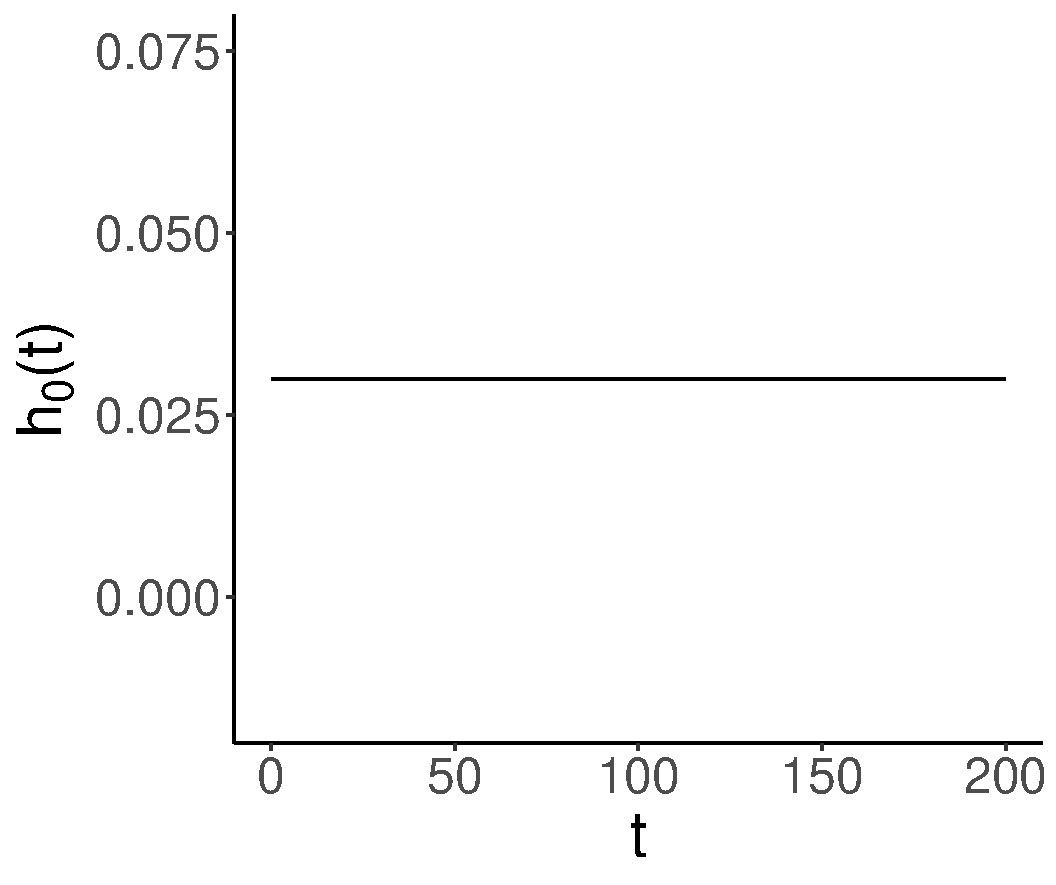
\includegraphics[width=2in]{cons_base.pdf}
%\caption{fig1}
\end{minipage}%
}%
\subfigure[baseline 2]{
\begin{minipage}[t]{0.33\linewidth}
\centering
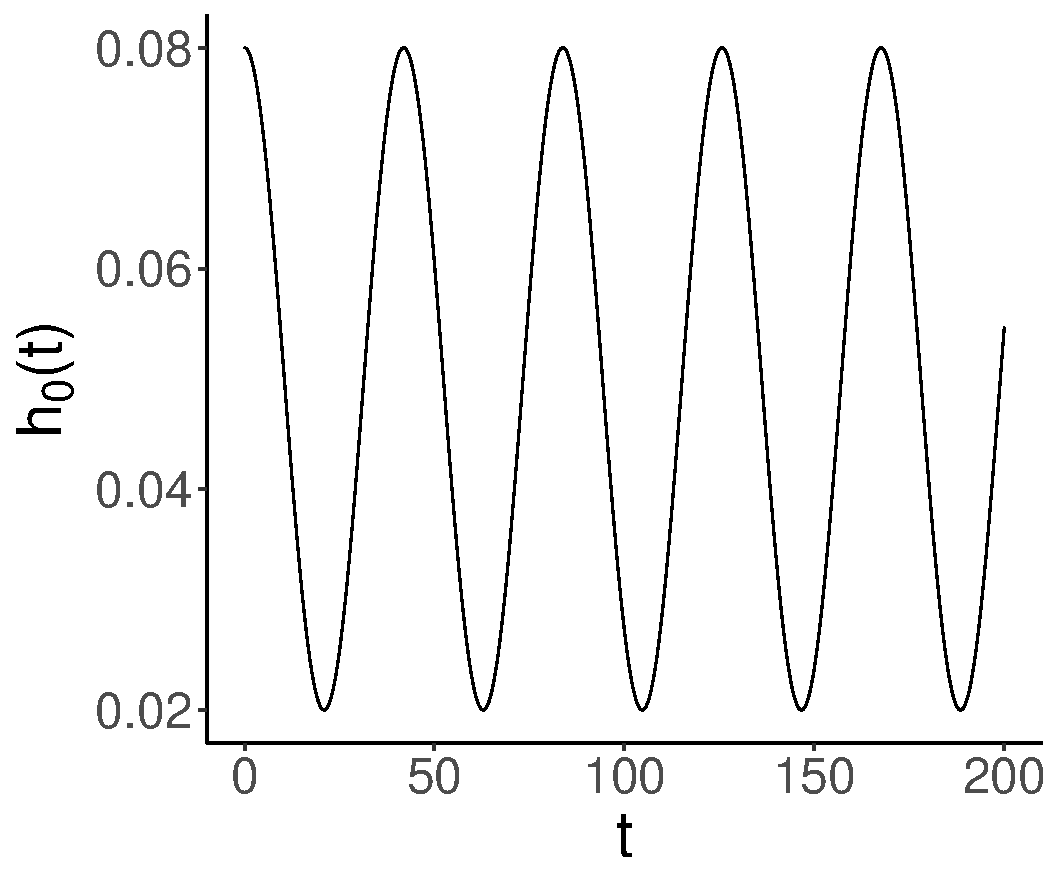
\includegraphics[width=2in]{regular_base.pdf}
%\caption{fig2}
\end{minipage}%
}%
\subfigure[baseline 3]{
\begin{minipage}[t]{0.33\linewidth}
\centering
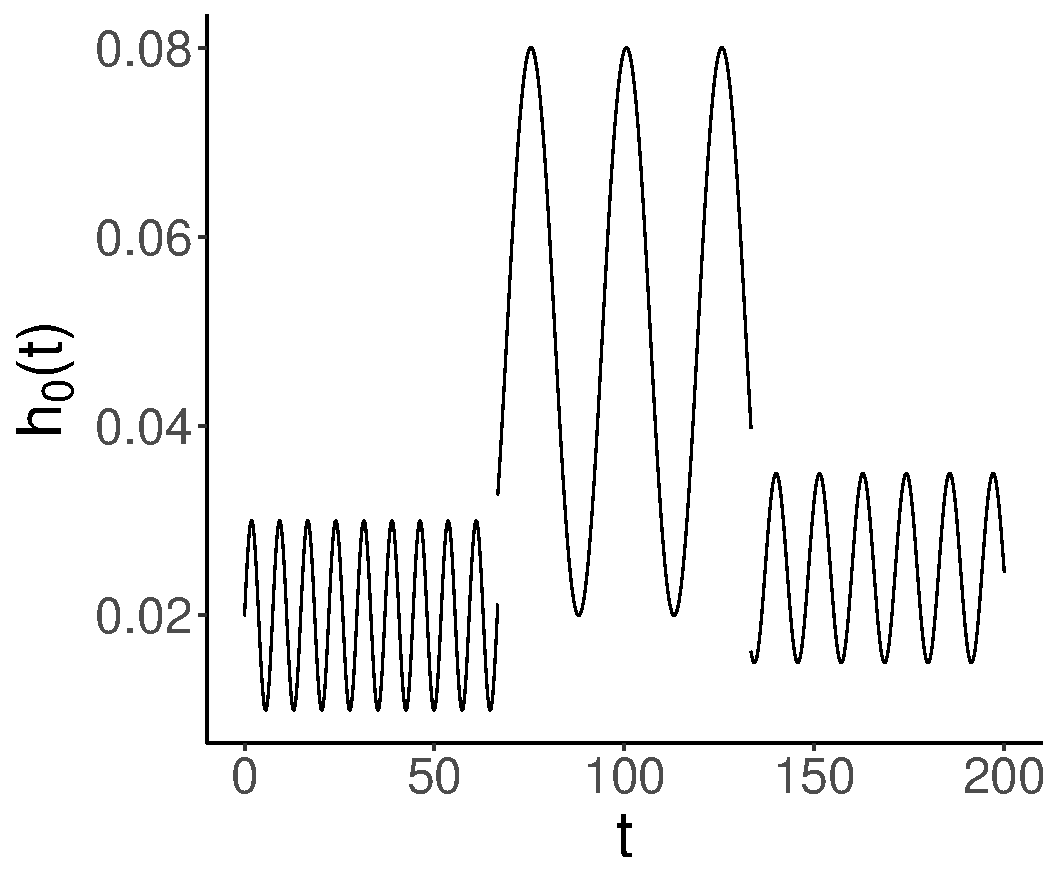
\includegraphics[width=2in]{com_base.pdf}
%\caption{fig2}
\end{minipage}
}%

\subfigure[covariate effect under 1]{
\begin{minipage}[t]{0.33\linewidth}
\centering
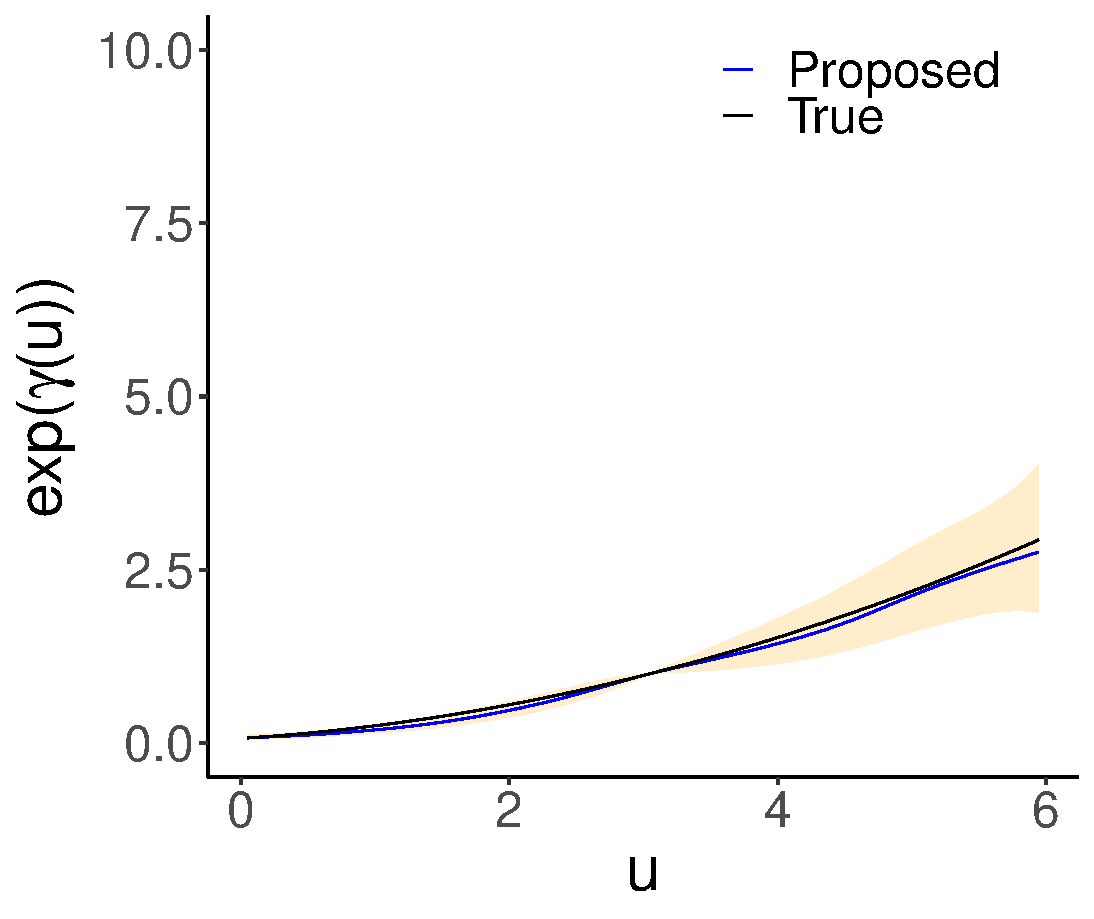
\includegraphics[width=2in]{cons_smooth.pdf}
%\caption{fig2}
\end{minipage}
}%
\subfigure[covariate effect under 2]{
\begin{minipage}[t]{0.33\linewidth}
\centering
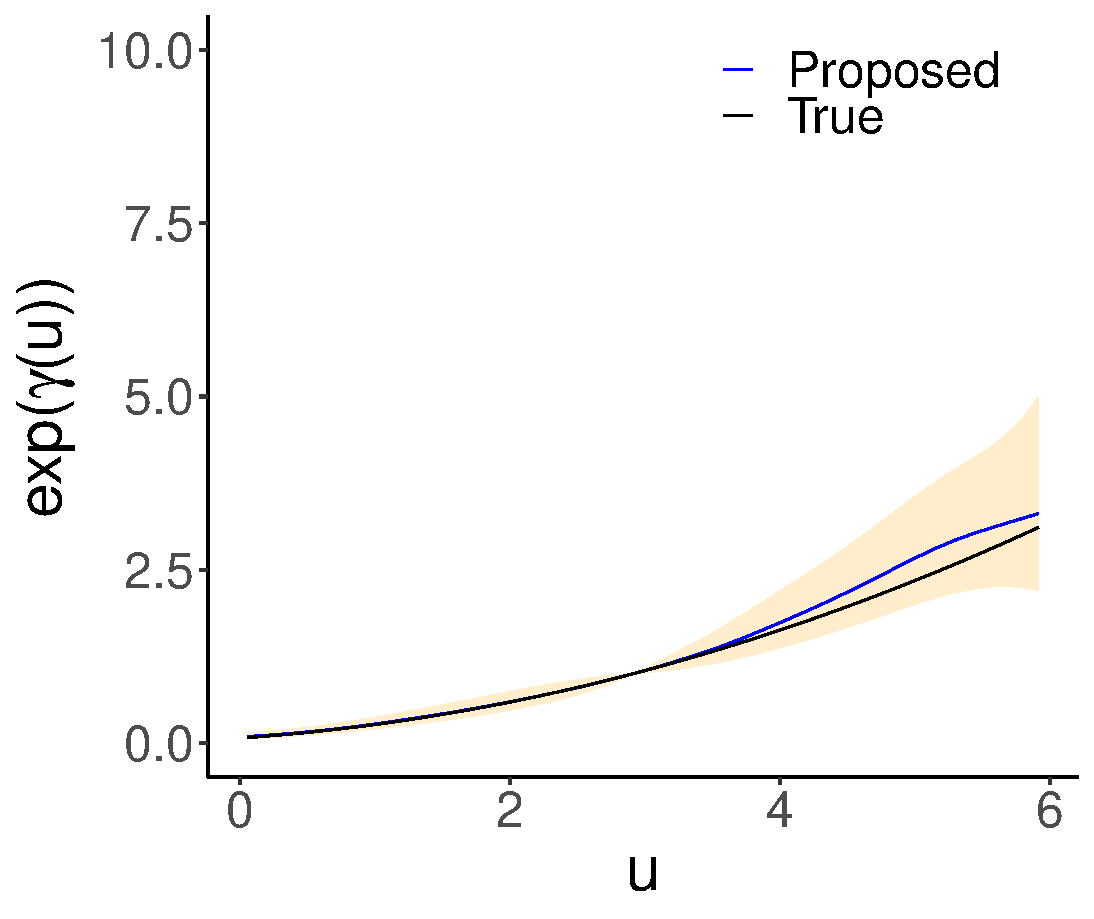
\includegraphics[width=2in]{regular_smooth.pdf}
%\caption{fig2}
\end{minipage}
}%
\subfigure[covariate effect under 3]{
\begin{minipage}[t]{0.33\linewidth}
\centering
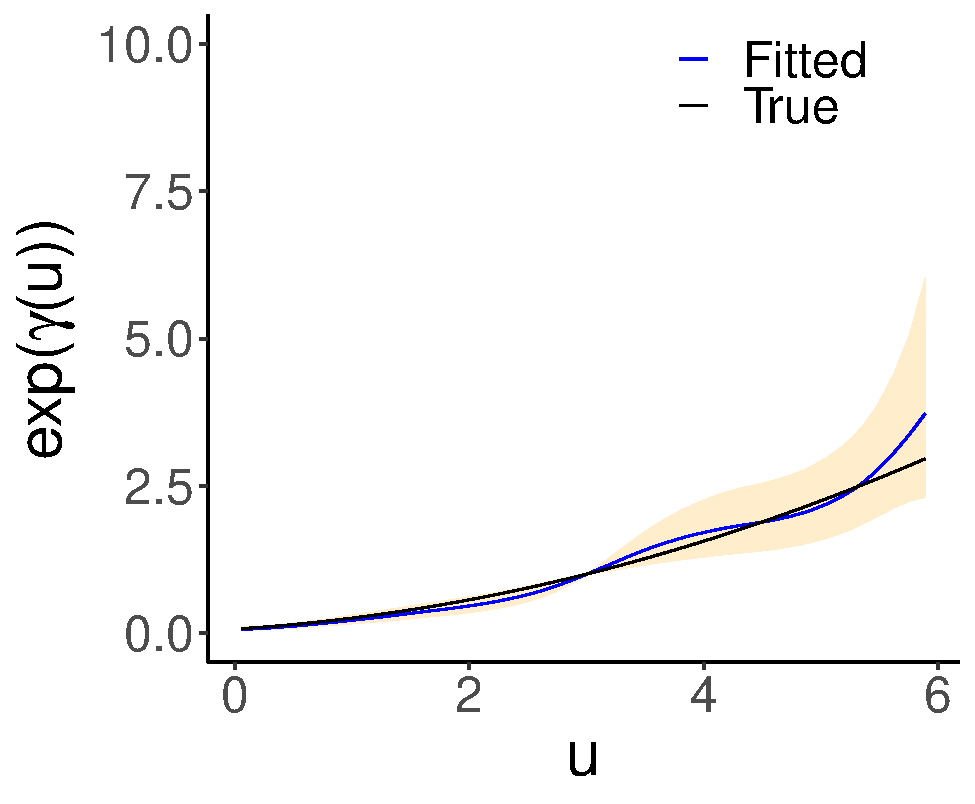
\includegraphics[width=2in]{com_smooth.pdf}
%\caption{fig2}
\end{minipage}
}%

\subfigure[variance parameter under 1]{
\begin{minipage}[t]{0.33\linewidth}
\centering
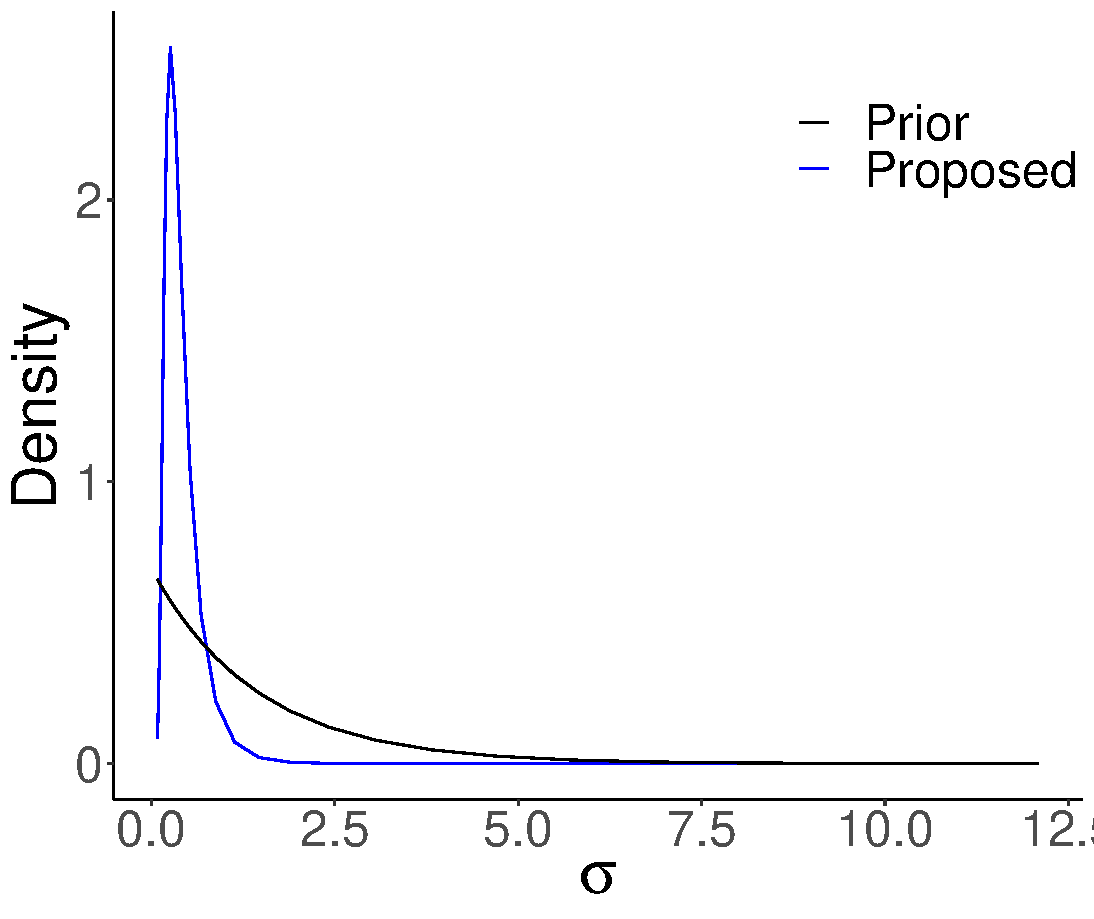
\includegraphics[width=2in]{cons_smooth_hyper.pdf}
%\caption{fig2}
\end{minipage}
}%
\subfigure[variance parameter under 2]{
\begin{minipage}[t]{0.33\linewidth}
\centering
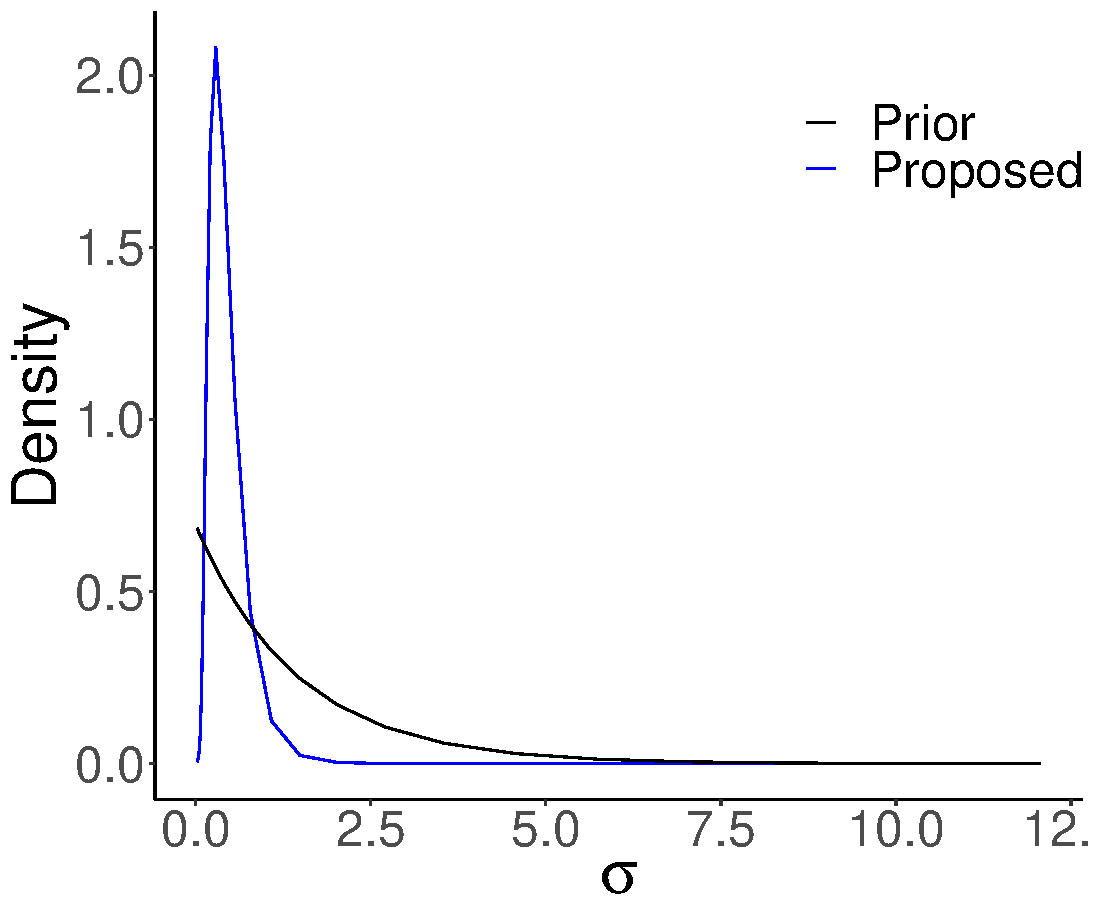
\includegraphics[width=2in]{regular_smooth_hyper.pdf}
%\caption{fig2}
\end{minipage}
}%
\subfigure[variance parameter under 3]{
\begin{minipage}[t]{0.33\linewidth}
\centering
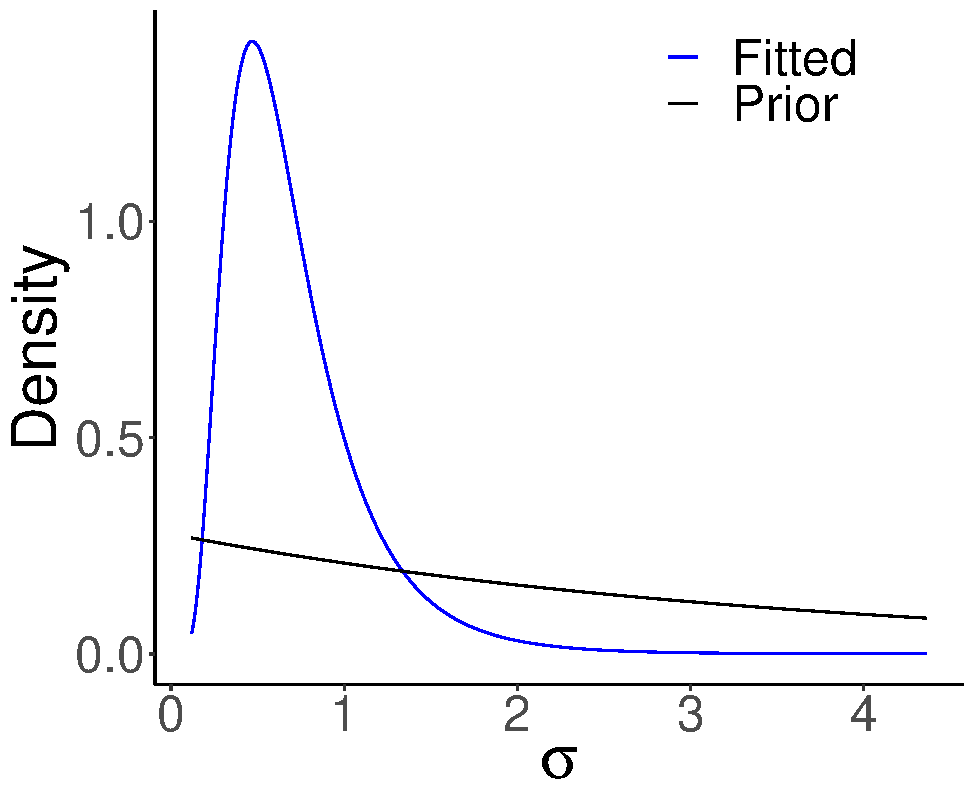
\includegraphics[width=2in]{com_smooth_hyper.pdf}
%\caption{fig2}
\end{minipage}
}%

\centering
\caption{Inferred covariate effects and variance parameters under different baseline hazard functions}
\label{fig:simulation1}
\end{figure}



\begin{figure}[ht]
\centering

\subfigure[baseline 1]{
\begin{minipage}[t]{0.33\linewidth}
\centering
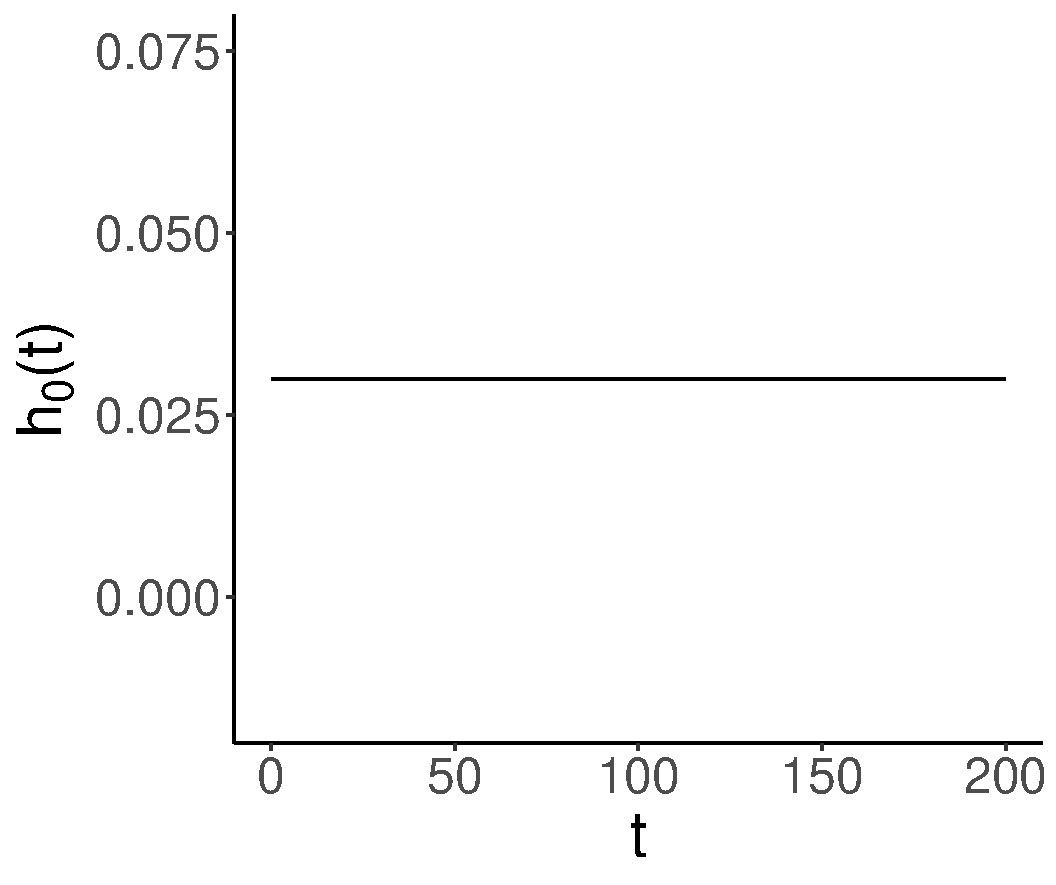
\includegraphics[width=2in]{cons_base.pdf}
%\caption{fig1}
\end{minipage}%
}%
\subfigure[baseline 2]{
\begin{minipage}[t]{0.33\linewidth}
\centering
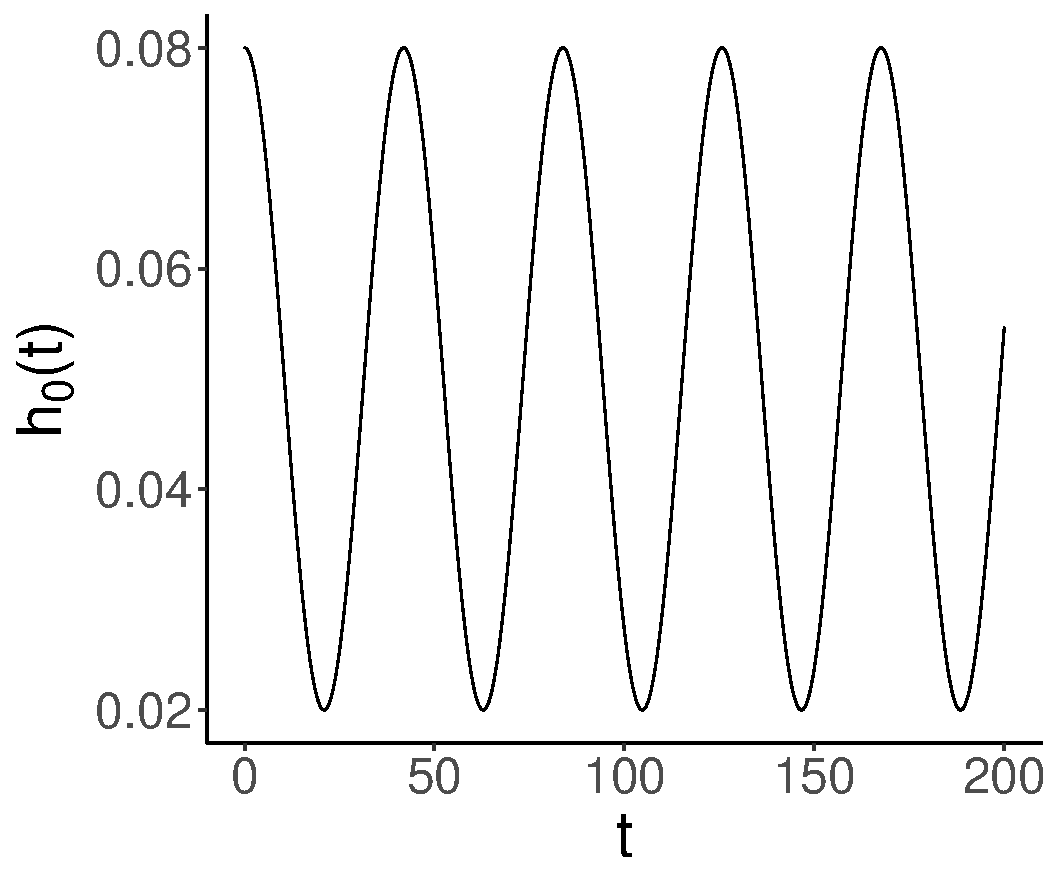
\includegraphics[width=2in]{regular_base.pdf}
%\caption{fig2}
\end{minipage}%
}%
\subfigure[baseline 3]{
\begin{minipage}[t]{0.33\linewidth}
\centering
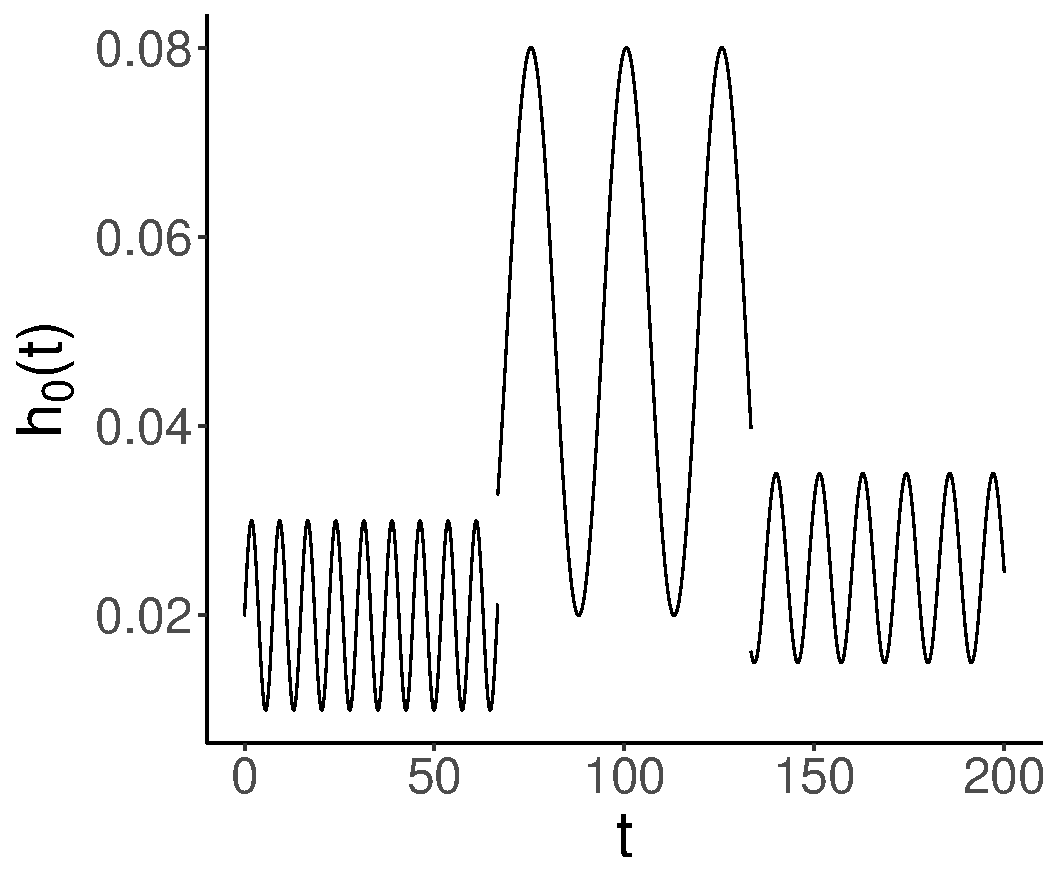
\includegraphics[width=2in]{com_base.pdf}
%\caption{fig2}
\end{minipage}
}%

\subfigure[covariate effect under 1]{
\begin{minipage}[t]{0.33\linewidth}
\centering
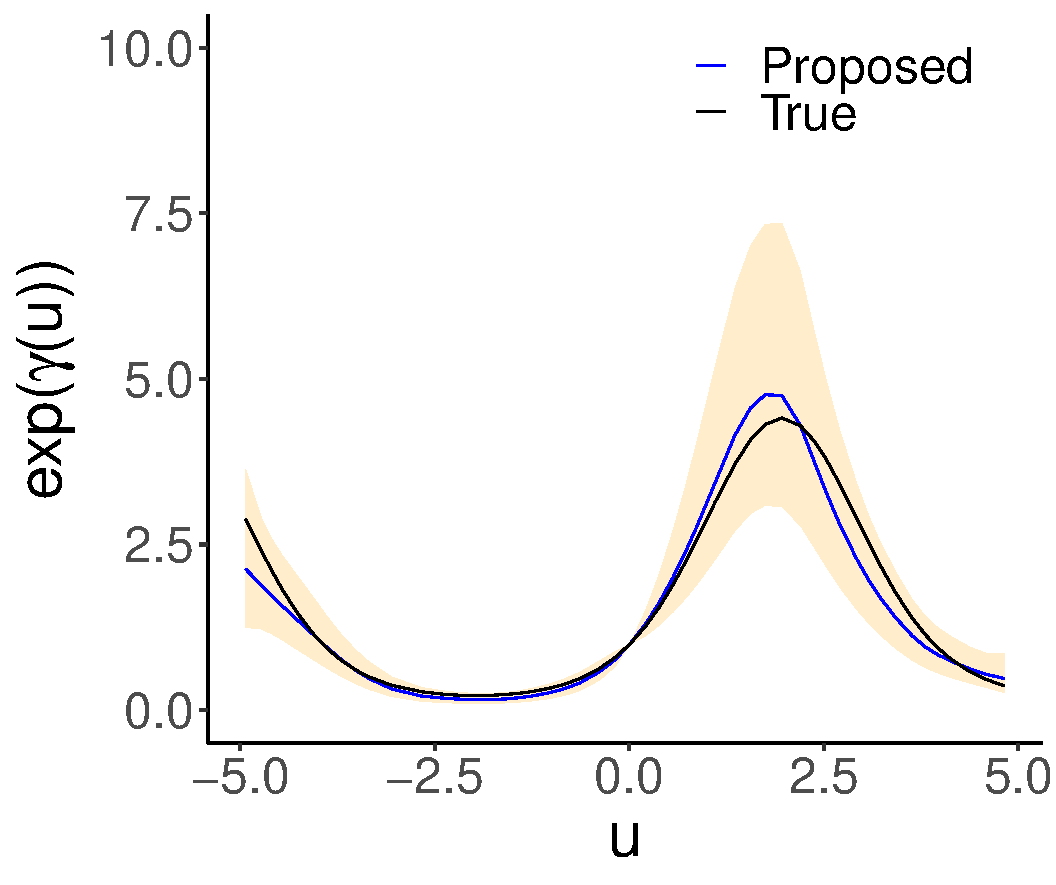
\includegraphics[width=2in]{cons_base_com_truth.pdf}
%\caption{fig2}
\end{minipage}
}%
\subfigure[covariate effect under 2]{
\begin{minipage}[t]{0.33\linewidth}
\centering
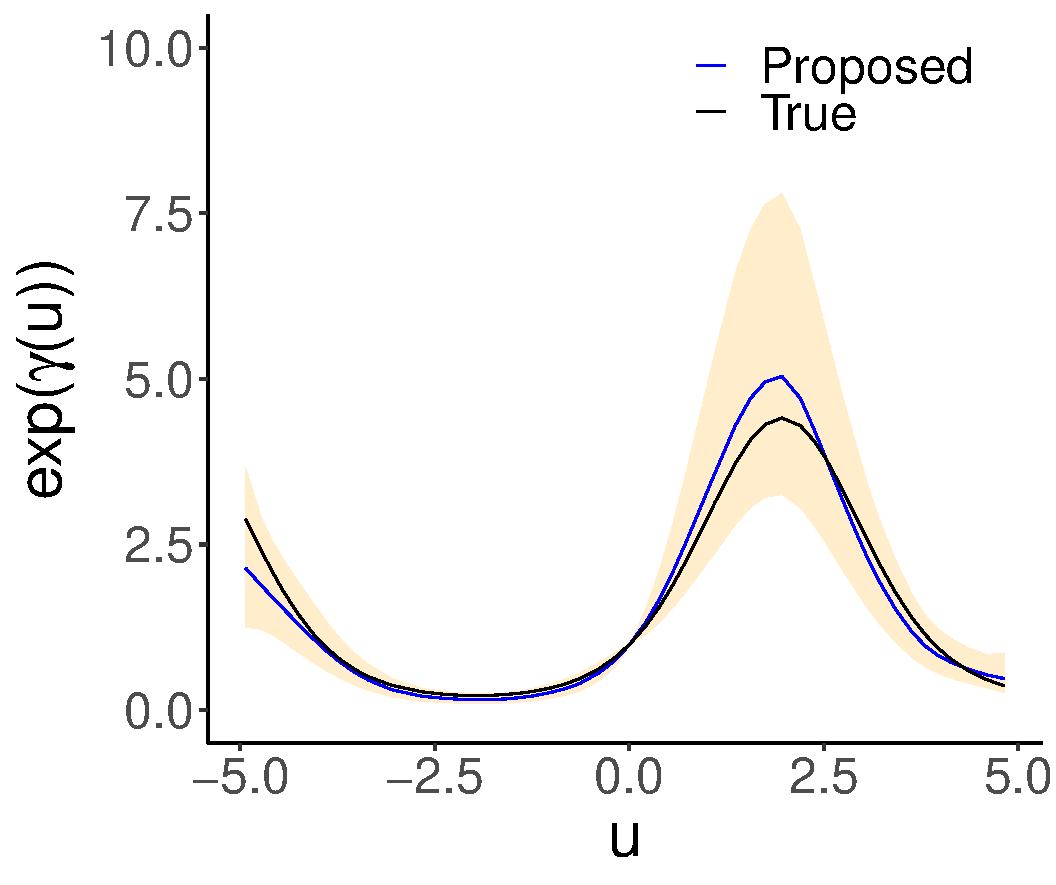
\includegraphics[width=2in]{regular_base_com_truth.pdf}
%\caption{fig2}
\end{minipage}
}%
\subfigure[covariate effect under 3]{
\begin{minipage}[t]{0.33\linewidth}
\centering
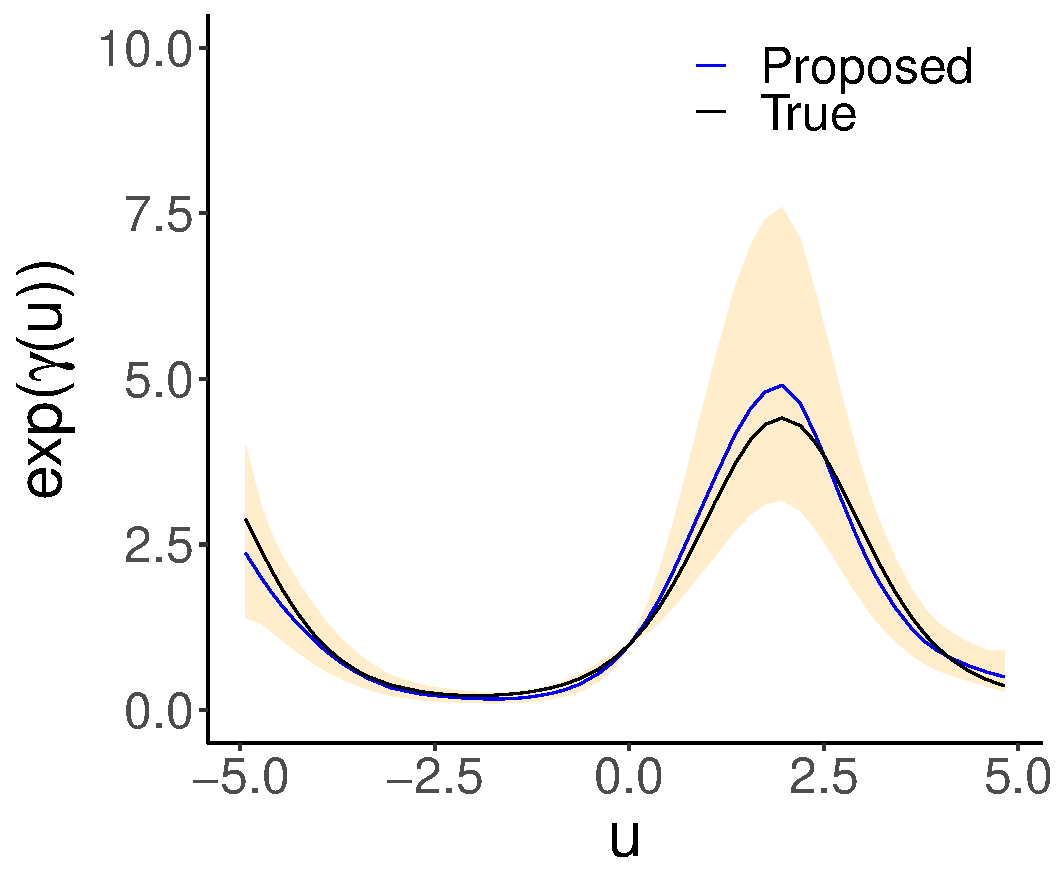
\includegraphics[width=2in]{com_base_com_truth.pdf}
%\caption{fig2}
\end{minipage}
}%

\subfigure[variance parameter under 1]{
\begin{minipage}[t]{0.33\linewidth}
\centering
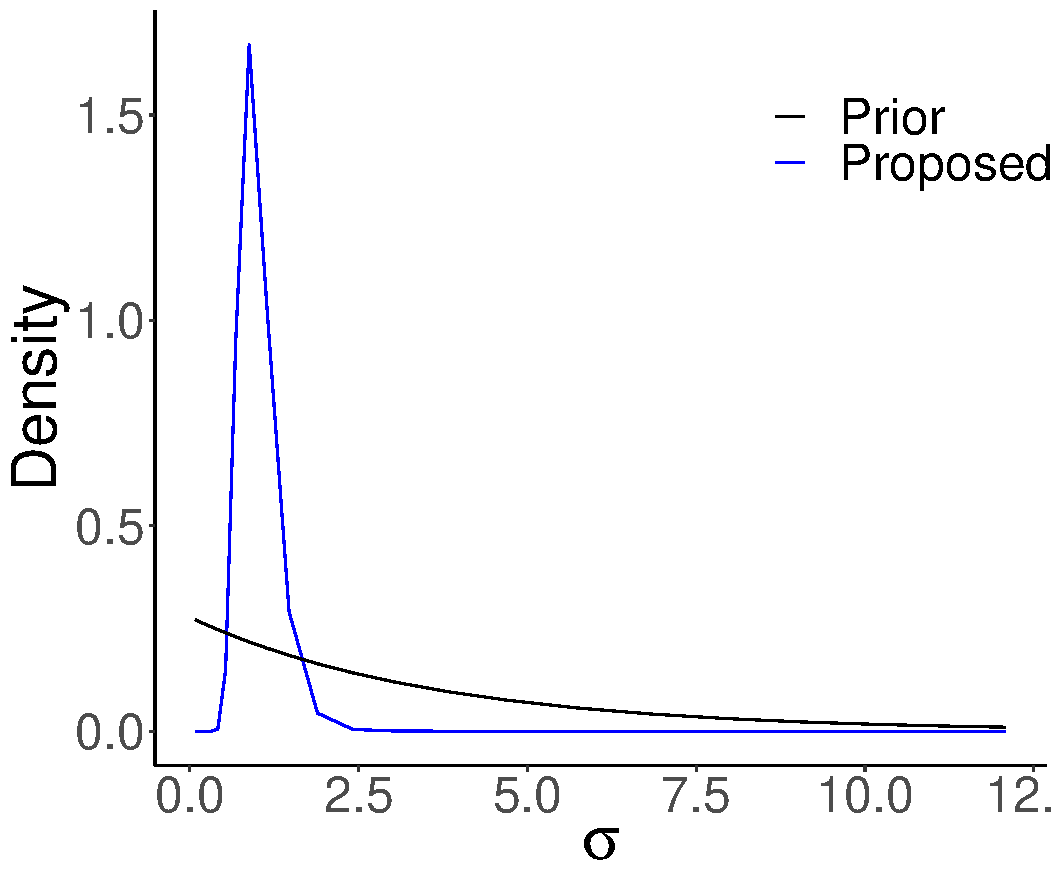
\includegraphics[width=2in]{cons_base_com_truth_hyper.pdf}
%\caption{fig2}
\end{minipage}
}%
\subfigure[variance parameter under 2]{
\begin{minipage}[t]{0.33\linewidth}
\centering
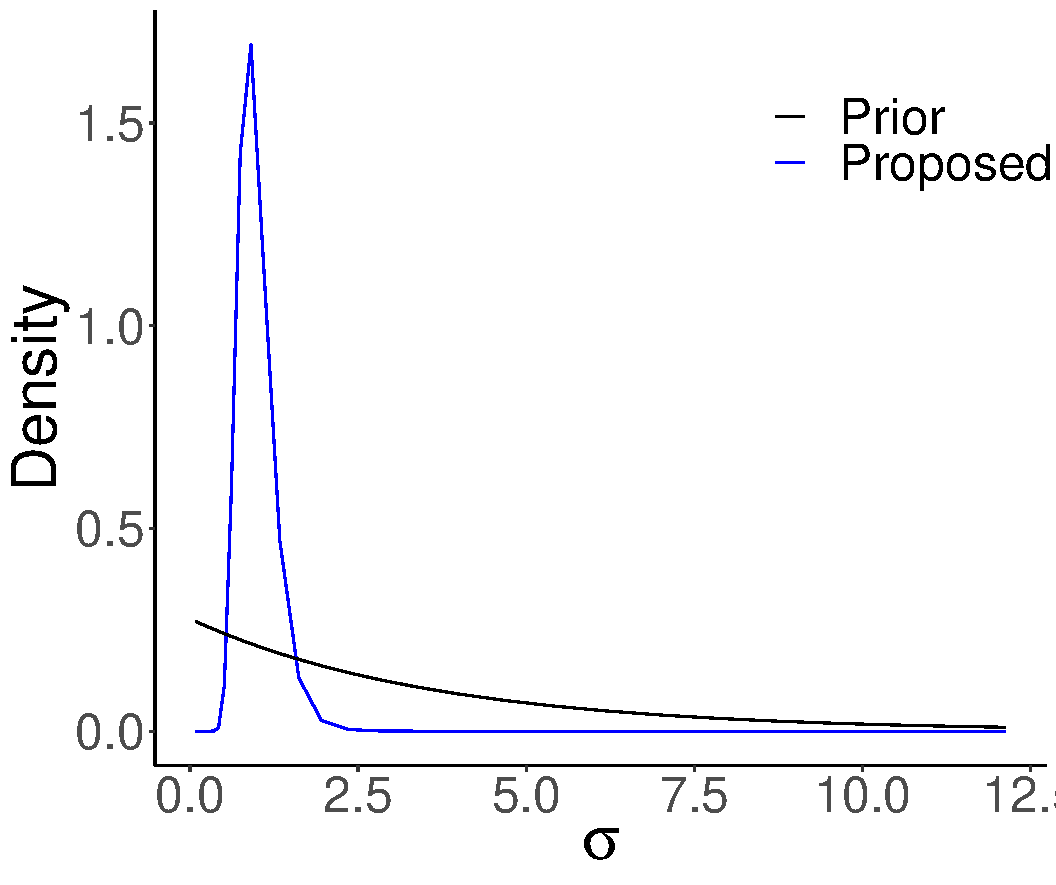
\includegraphics[width=2in]{regular_base_com_truth_hyper.pdf}
%\caption{fig2}
\end{minipage}
}%
\subfigure[variance parameter under 3]{
\begin{minipage}[t]{0.33\linewidth}
\centering
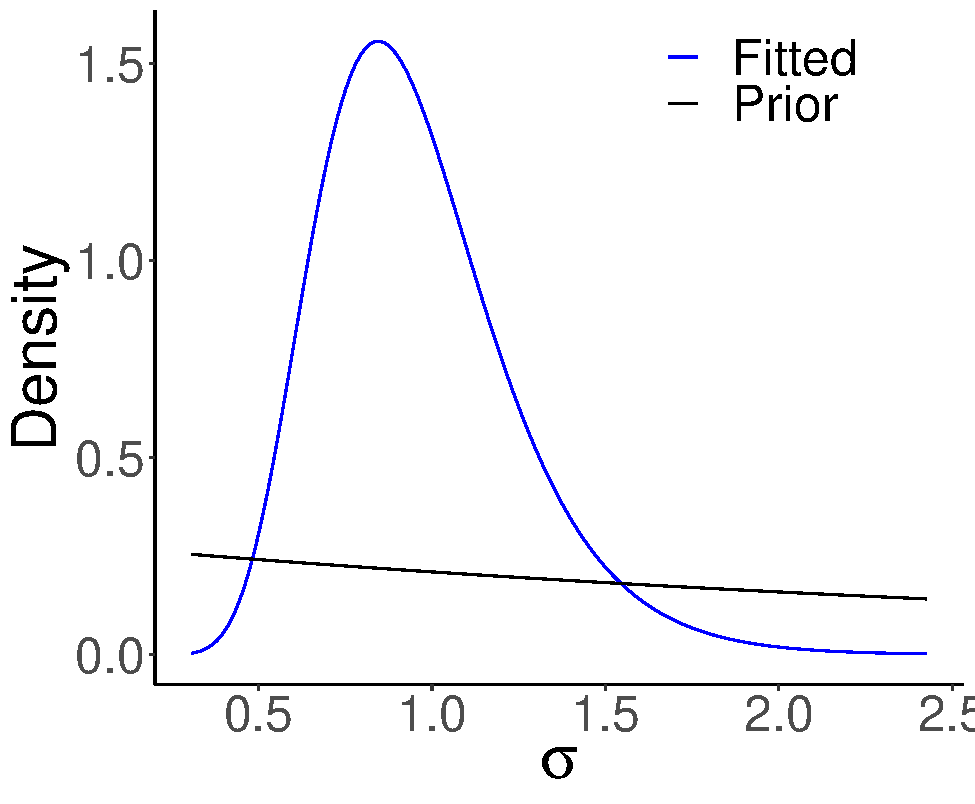
\includegraphics[width=2in]{com_base_com_truth_hyper.pdf}
%\caption{fig2}
\end{minipage}
}%

\centering
\caption{Inferred covariate effects and variance parameters under different baseline hazard functions}
\label{fig:simulation2}
\end{figure}



\begin{figure}[ht]
\centering
\subfigure[Posterior effect of \texttt{tpi}]{
  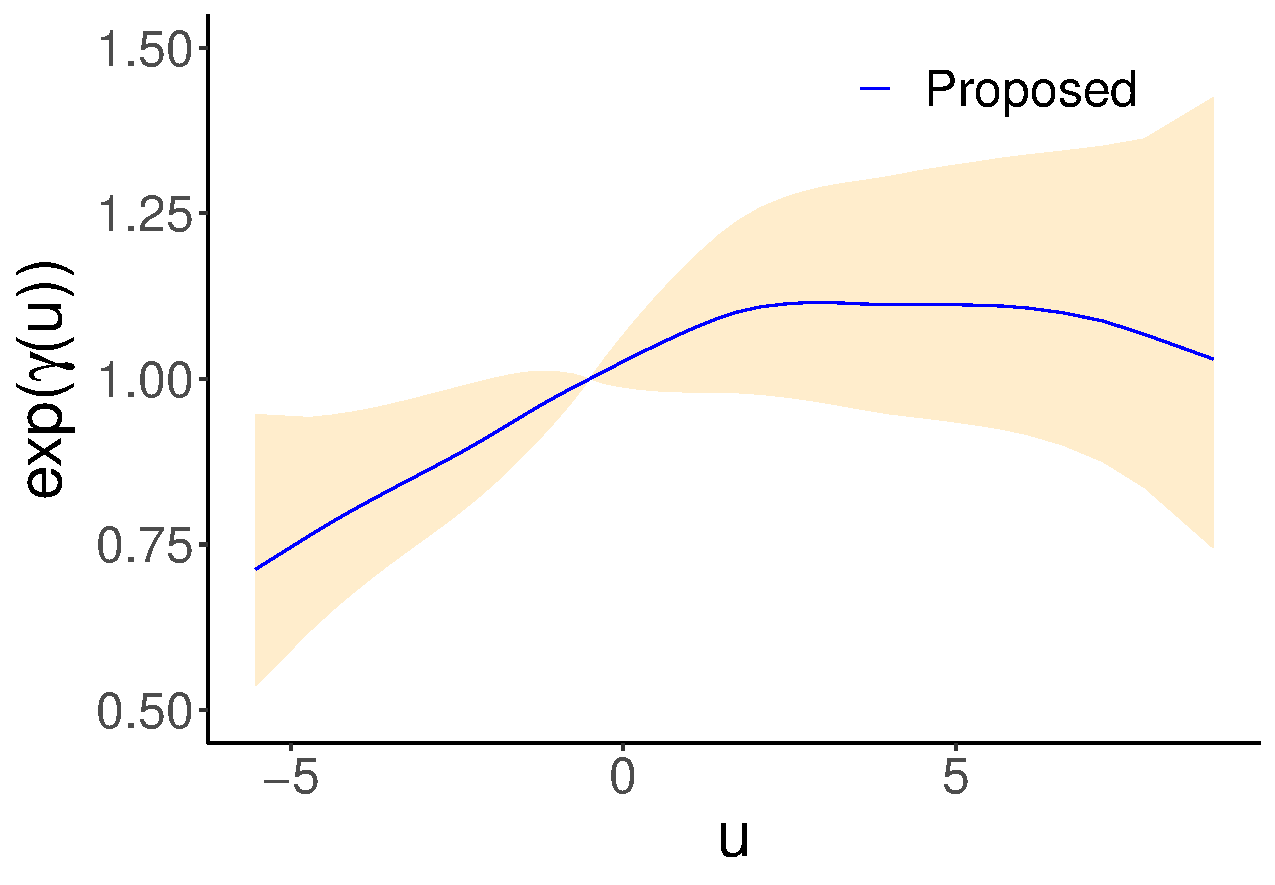
\includegraphics[width=0.45\textwidth,height=2.5in]{leuk_smooth.pdf}
}
\subfigure[Posterior distribution of $\sigma$]{
	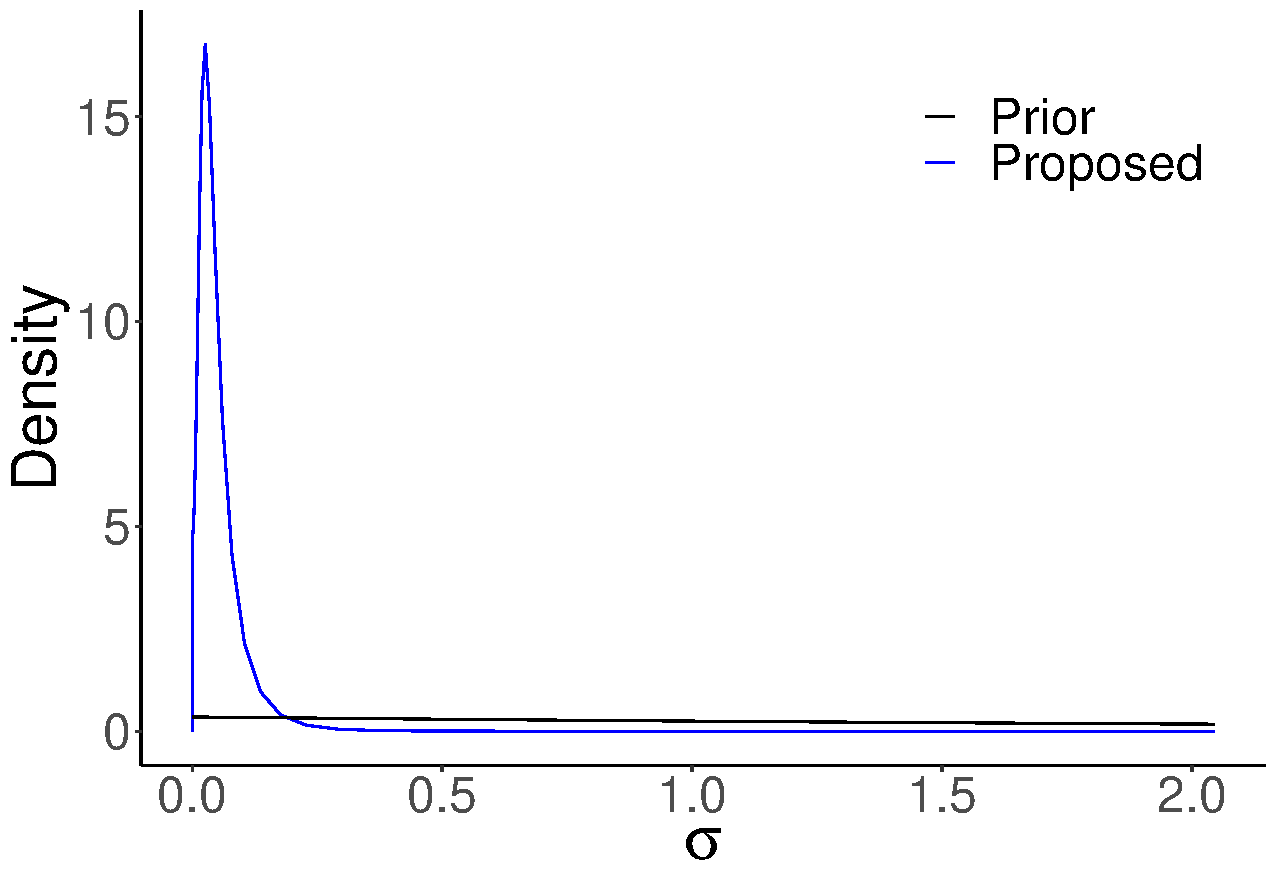
\includegraphics[width=0.45\textwidth,height=2.5in]{leuk_hyper.pdf}
}
\caption{Results for the Leukaemia data in section \ref{subsec:leuk}. (a): posterior mean (blue) and $95\%$ credible interval (shaded) using our method (b): prior (black) and approximate posterior distribution for $\sigma$ using our method (blue).}
\label{fig:leuk}
\end{figure}

\begin{figure}[ht]
\centering
\subfigure[Posterior distribution of $\sigma$]{
	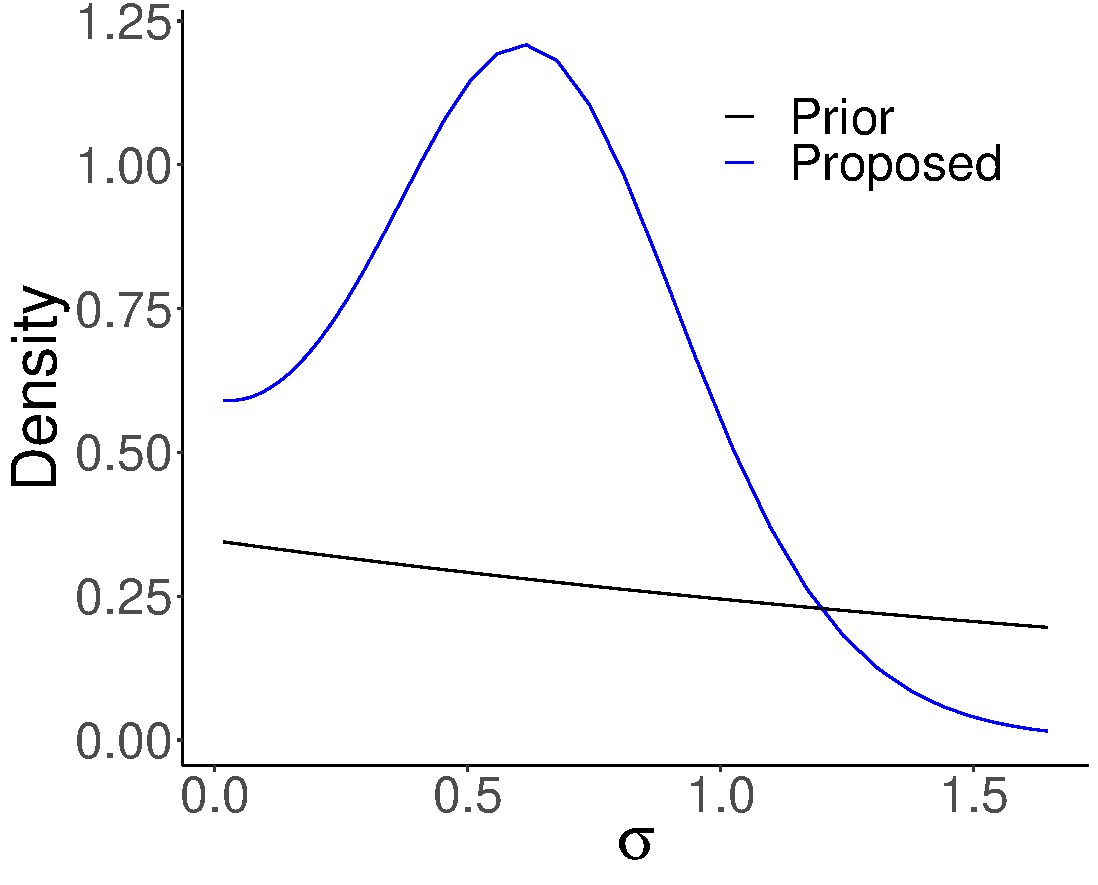
\includegraphics[width=0.45\textwidth,height=2.5in]{kidney_hyper.pdf}
}
\caption{Posterior distribution for the between-subject standard deviation by our method (blue) and its prior (black), for the kidney data in section \ref{subsec:kidney}.}
\label{fig:BetweenSubjectSD}
\end{figure}


\end{document}

